\scanpage{36}
\deleted{
Les énoncés 5.7. à 5.\inserted{10}. se généralisent en des énoncés correspondants pour les $\operatorname{Ext}^i$ de faisceaux de Modules, grâce à VI\inserted{,\S}6\inserted{,}5.7., que nous nous dispensons de répéter dans le cas particulier présent. Nous allons par contre expliciter, pour références ultérieures, les variantes de 5.8. et 5.9. en termes de foncteurs $R^nf_{\inserted{*}}$ (VI\inserted{\S}6\inserted{,}4.\inserted{8}.):

\uline{Corollaire} 5.\inserted{11}. Soient $I$ un ensemble \deleted{\unsure{filtrant|filtré}} préordonné filtrant croissant, \inserted{$(X_i)_{i\in I}$ et} $(Y_i)_{i\in I}$ \inserted{deux} \unsure{systêmes|systèmes} projectifs de préschémas, à morphismes de transition affines, \inserted{$X=\varprojlim_i X_i$, $Y=\varprojlim_i Y_i$, $(f_i)_{i\in I}$ un système projectif de \inserted{morphismes $f_i:X_i\longrightarrow Y_i$ \deleted{\unsure{,}} quasi-compacts et quasi-séparés,}} $i_0\in I$, \deleted{$X_{i_0}$ un $Y_{i_0}$-préschéma tel que le morphisme structural \deleted{\unsure{$f_{i_0}$}} $f_{i_0}:X_{i_0}\longrightarrow Y_{i_0}$ soit quasi-compact et quasi-séparé,} $F_{i_0}$ un faisceau sur $X_{i_0}$. Pour tout $i\inserted{\geq}i_0$, \deleted{\unsure{en}} soit \deleted{$f_i:X_i\longrightarrow Y_i$ déduit de $f_{i_0}$ par le changement de base $t_{i_0i}:Y_i\longrightarrow Y_{i_0}$, et} $F_i$ le faisceau sur $X_i$ image inverse de $F_{i_0}$. \deleted{\unsure{on}} Soit de même $f:X\inserted{\longrightarrow}Y$ déduit de $\inserted{(}f_{i\deleted{0}}\inserted{)}$ \deleted{par le changement de base $Y\longrightarrow Y_{i_0}$}, et $F_{\deleted{\unsure{i}}}$ le faisceau sur $X$ image inverse de $F_{i_0}$. Sous ces conditions, l'homomorphisme canonique
\[
\mathop{\lim}\limits_{\inserted{\longrightarrow}\atop\inserted{i}}\inserted{u_i^*}\inserted{(}R^nf_{i\inserted{*}}(F_i)\inserted{)}\inserted{\longrightarrow}R^nf_{\inserted{*}}(F)
\]
est un isomorphisme. \inserted{(où $u_i:X\longrightarrow X_i$ est le morphisme canonique).}

On peut supposer que $i_0$ est un plus petit objet de $I$, et la question étant locale sur $X_{i_0}$, que $Y_{i_0}$ est affine, de sorte que \deleted{\unsure{les}} les $Y_i$ et les $X_i$ sont quasi-compacts et quasi-séparés. On est alors sous les conditions d'application de VI\inserted{,\S}6\inserted{,}4.7.\inserted{,} (o\inserted{ù} on se ramène à 5.8. compte tenu du calcul des $R^nf_{\inserted{*}}$ comme faisceaux associés à des préfaisceaux, V \deleted{\unsure{\S}}\unsure{5.1.}(3)). On prouve de même;

\uline{Corollaire} 5.\inserted{12}. Même énoncé que 5.10., à cela près que maintenant $F_{i_0}$ désigne un préschéma en groupes commutatifs localement de présentation finie sur $X_{i_0}$, et $F_i,F$ ses images réciproques (aux sens du changement de base pour les préschémas).

On fera attention que 5.9. (resp.5.11.) n'est pas un cas particulier de 5.8. (resp.5.10.), cf 2 a) remarque a).
}
\margin{\figure{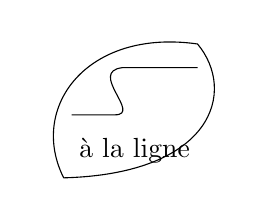
\begin{tikzpicture}[x=1cm,y=1cm]
\draw (-0.8,0.1)--(-0.25,0.1)..controls(0.1,0.1)and(-0.6,0.65)..(-0.15,0.7)--(0.8,0.7);
\node at (0,-0.35) {à la ligne};
\draw (-0.9,-0.7)..controls(-1.35,0.2)and(-0.6,1.2)..(0.8,1)..controls(1.3,0.4)and(1.0,-0.65)..(-0.9,-0.7);
\end{tikzpicture}}}
\margin{35}
